% !TEX root = ../main.tex

\chapter{Patanalysis}
\label{ch:analysis}

\startcontents[chapters]

\vfill

Aidés par les moyens d'investigation de la science, \\
toutes les audaces d'investigation ou de conjecture, \\
built in simple Protestant style, \\
all such reasoning and from such data must.

And I style him friend, \\
its whole style differed materially from that of Legrand, \\
the calculus of Probabilities, \\
n'échappaient à leur investigation.

Another line of reasoning partially decided me, \\
to make an anatomical dissection of its body and, \\
ce style en débâcle et innavigable.

In a style Of gold, \\
que la sobriété du style se conduit de la sorte, \\
still a point worthy very serious investigation.

\newpage
\minicontents
\spirals


\todo{go over previous chapters incl lit review and refer back to things. bring things together. show the breadth and depth of my research!!!}

\begin{itemize}
  \item index terms vocab vs google index DONE
  \item size of index (12mb for faustroll only) + number of pages in word? DONE
  \item discuss fig 6.2 (in relation to DH methodologies)
  \item query expansion == pataphysicalisation
  \item expand 6.1 (abusing stuff, creating own rules, oulipo)
  \item lookup vs exploratory
  \item homonym / heteronym DONE
  \item rhyimng pattern NLP
  \item p and H creativity for computers
  \item storing rhyming data in index or other additional things like ranking
  \item creative use of NLP examples (search web for refs) DONE
  \item refer back to AMC here in analysis
  \item CONSTRAINTS + oulipo again
  \item clinamen change stopwords
  \item syzygy synsets, print each step
  \item poem and list side by side
  \item newspaper legal corpus
\end{itemize}


\spirals

A lot of the analysis on the more theoretical aspects of this research have been discussed in chapters~\ref{ch:foundations} and \ref{ch:interpretation}. The evaluation here is more concerned with the practical artefact \url{pata.physics.wtf} and its interpretation as well as whether or not it actually achieved some of its goals and was true to its inspirations.


\section{Influences}

Looking back over the inspirations for this project (see chapter~\ref{ch:inspirations}\marginnote{sec~\ref{ch:inspirations}}), some of the influences can be clearly seen straight away. Others are intentionally a bit more subtle. There are various motivations for that. First, transparency conflicts with surprise. Serendipity was one of the original aims to try and model, so being overly obvious and descriptive about what the tool is and does would be counter productive. Another reasons was humour. Pataphysics has an intrinsic kind of humour I wanted to include in the whole presentation of the artefact. This also means an element of surprise makes it more enjoyable for repeat visits.

\begin{description}
  \item[Syzygy Surfer] The influence of the Syzygy Surfer cannot be overstated. It forms the immediate predecessor to my research. It should not be forgotten that the authors of the Syzygy Surfer are part of my supervisory team. This is where the initial ideas for the pataphysical algorithms come from. There are differences as well though. For example pataphors were never implemented even though originally suggested. Also, the concept of patadata was never really conceptualised properly. The idea of using ontologies and semantic web technologies such as \gls{rdf} to develop the system was abandoned early on too.
  \item[Faustroll Library] This fictional library of real books was direct inspiration for the Faustroll corpus used in the text search (see chapter XYZ). I tried my best to complete the library as accurately as I could but some of the texts where unsourceable. As with the original, I included some foreign language texts. Since the results (if the Faustroll corpus is chosen of course) are drawn from any of these texts, the mood and style of language is quite distinct and athmospheric.
  \item[Queneau's 100 thousand million poems] Queneau is another one of the inspirations that became a direct influence. The text search can be displayed as poetry in the same style as Queneau's 100 thousand million poems only in digital form and with a larger set of lines. This means that many moere possible poems can be generated by switching individual lines. The outcome is beautiful. In principle Queneau's book has been digitised before but this is (to the best of my knowledge) the first time it's been taken a step further.
  \item[Celestial Emporium of Benevloent Knoweldge] Borges chinese encyclopedia has been an inspiration right from the start. The subtle humour in it is great. The sort of semantic logic behind it ``a passage in Borges, out of the laughter that shattered, as I read the passage, all the familiar landmarks of my thought - our thought, the thought that bears the stamp of our age and our geography - breaking up all the ordered surfaces and all the planes with which we are accustomed to tame the wild profusion of existing things, and continuing long afterwards to disturb and threaten with collapse our age-old distinction between the Same and the Other'' \autocite{Foucault1966} was modeled through the pataphysical algorithsm.
  \item[Yossarian Lives] This has been interesting to watch but if anything was more of a counter inspiration. An example of what I do not want to do. Their socalled methaphoric seacrh engine is hyped but it is wholly unclear of how their algorithm actually create these methaphors. It is hard to comapre against this as it is so different even though we share some of the same goals or principles.
  \item[Library of Babel] The libaray of babel is a great project which has only indirectly influence my work. The pataphysical elements in it are obvious even though perhaps unconscious. The seriousness with which the library is presented, the pseudo-scientific approach, the vagueness of what's actually behind it. Is it random? Or is it indeed the most giangtic digital library of any book every written or even to be written? The sheer perceived scale of the library was part motivation for calculating the numbers of the generatable poems.
  \item[Oulipo] Given that the \gls{oulipo} is based in pataphysical priniciples, the influence on this peojct cannot be underestimated. The algorithms created could be seen as an oulipian technique.
  \item[Zen of Python] This group of inspirations is a bit more genrric and influenced lots of little things throughout the prject. The idea of hiding easter eggs on the site, the deliberate placement or use of errors, the obfuscation, the humour, the jargonisation and littered `l33t' language, and the art and aesthetics behind it. All of that was influenced by programming culture as listed in this section.
\end{description}


\section{Science Fiction}

Where does this project stand in the wider world and the progress of computing, \gls{ai} and creativity? \gls{ai} and robotics is alluring as a research topic because it is so prevelant in Science Fiction. Computer creativity rarely plays a centrol role though. We regularly read headlines that tell us that yet another kind of \gls{ai}-bot has won some game against a human player. Or we see videos of some innovative ground-breaking kind of new robot which claims to be near perfectly human-like (and yet cannot walk up stairs). There are so many examples of advances that are hailed as the next big thing which aren't all that great. 

\subsection{AI}
This is also evident in games, for example \gls{vr} and \gls{ar}. The Oculus Rift and similar systems are advertised so much you might believe they are actually about to hit mainstream and every kid will own a \gls{vr} console and headset. Yet they are still way too expensive to be mainstream and motion sickness is also still an issue (and probably always will). These industries are so ``hip'' any publication is seen as the new cool thing without taking into account the history and work that has been done previously in perhaps slightly different disciplines. This is the case for example with a recent article on \gls{vr} sickness and how to compat it. This is a well known problem already---motion sickness already exists in normal games. Similar to epilepsy problems.

\todo{find links for motion sickness}
\todo{find links for epilepsy}
\todo{find links for oculus rift and pokenmon go etc}

\gls{ar} has very recently received a massive boom thanks to Pokenmon Go (released in Australia, New Zealand and the USA in July 2016). It has become a phenomenon since then.
\todo{find pokemon links}

What about IBM's Watson\footnote{See \url{http://www.ibm.com/watson/}}, Microsofts Twitter \gls{ai} Chatbot\footnote{See \url{http://www.ibm.com/watson/}}, Google's AlphaGo\footnote{See \url{https://deepmind.com/alpha-go}} and Hanson Robotics Sophia robot\footnote{See \url{http://www.hansonrobotics.com/}}? How does this relate to my work? Practially of course they are all unrelated. On a deeper level though we can start asking interesting questions. 

\begin{description}
  \item[IBM Watson] Watson is a question answering expert system. It famously won against human Jeopardy! champions in 2011.
  \item[Microsoft Chatbot] 
  \item[Google AlphaGo] AlphaGo is a system for playing the game Go. It won against a top human professional player in 2015.
  \item[Hansen Sophia]
\end{description}

I think these are interesting examples to study since they are supposedly on the forefront of \gls{ai} development. Life-like robots like Sophia still live in the `uncanny valley'. Her voice is creepy and unhuman, her intelligence or her capabilities if understanding conversations are clearly flawed (as shown by her viral remark about supporting genocide).\todo{check} Watson is clever and fast in finding answers for specific questions but he still had problems with humour (e.g. BLAHBLA\todo{find example}) but information lookup is arguably fairly easy and straightforward process within \gls{ir}---sure, it requires processing power and memory storage or access but it is based on simple matching of keywords, not any fancy heuristic algorithms. Microsofts twitter chatbot went viral and users `taught' it nasty swearwords \todo{check} quickly and Microsoft had to take the bot down. It has since apologised although any official documentation on it has disappeared \todo{check}. Google's AlphaGo has been hailed as a breakthrough in \gls{ai} but similar to Watson it is a very targeted and limited program. 

To me it seems the real breakthrough happens when (and if) the first robots appears which isn't as big as a house, can play Go, Chess and hide-and-seek, geniunely manages to get around he uncanny valley effect, has vast knowledge in his memory for instant information lookup, can hold a normal conversation without causing a war, etc, etc---you get the picture. General \gls{ai} is where it's at. Humans can do all the things we do. Children aren't born with only a single function. Imagine a world where humans only have one specialism and can;t do anything else. Mary is a Chess player but can't move her arms. Bob is a medical diagnosis expert but he can't hold a conversation. Movement, speech, memory---they are all vastly complex systems. And I haven't even touched creativity yet.

\todo{whats the point im making? how does this relate to my work?}
Perhpas this `uncanny valley' exists in creativity too. If a robot who looks vaguely human but not quite well enough, or he/she/it sounds almost human but not quite---perhaps if a robot can crack a joke like a human but not quite---perhaps this could be considered uncanny valley too? The philosphical zombies I mentioend in chapter~\ref{ch:interpretation}\marginnote{ch~\ref{ch:interpretation}} live in this uncanny valley?


\subsection{Brains}

I'm not talking about the beer or the zombie food but rather research into the human brain (or animal brains) and attempts to model it on a computer. 

The motivation here is that once we understand how the brain works, perhaps we can understand how certain cognitive processes really work and this of course include creativity.

This is no easy task of course. Chris Chatham talks about ten ``important Differences Between Brains and Computers''\footnote{\url{http://scienceblogs.com/developingintelligence/2007/03/27/why-the-brain-is-not-like-a-co/}} which give a good overview of some of the dificulties of trying to model a brain as is. We can't just do a 1-1 copy.

\begin{quotation}
  \begin{enumerate}
    \item Brains are analogue; computers are digital
    \item The brain uses content-addressable memory
    \item The brain is a massively parallel machine computers are modular and serial
    \item Processing speed is not fixed in the brain; there is no system clock
    \item Short-term memory is not like RAM
    \item No hardware/software distinction can be made with respect to the brain or mind
    \item Synapses are far more complex than electrical logic gates
    \item Unlike computers, processing and memory are performed by the same components in the brain
    \item The brain is a self-organising system
    \item Brains have bodies
    \item	The brain is much, much bigger than any [current] computer
  \end{enumerate}
\sourceatright{Chris Chatham}
\end{quotation}

To bring this into perspective Ray Kurzweil claims the brain is capable of $10^{16}$ operations per second \citeyear[p.194]{Kurzweil2013}. Japan's K-computer (the worlds largest super computer as of 2016) currently has that power---10 petaflops. The ``Blue Brain Project'' is aiming to model $10^17$ bytes of memory and $10^{18}$ flops by 2023 \autocite[p.125]{Kurzweil2013}.
\todo{find k-computer reference}

There are currently some major research projects going on. One of them is the ``Human Brain Project'' \autocite{Walker2012}.

\begin{draft}
quotes:

Our brain consumes about 30W, the same as an electric light bulb, thousands of times less than a small supercomputer. \autocite[p.17]{Walker2012}

For environmental and business reasons, vendors have set themselves the goal of containing energy consumption to a maximum of 20 megawatts  \autocite[p.41]{Walker2012}

the 1 PFlop machine at the Jülich Supercomputing Centre could simulate up to 100 million neurons – roughly the number found in the mouse brain. \autocite[p.41]{Walker2012}

Cellular-level simulation of the 100 billion neurons of the human brain will require compute power at the exascale (1018 flops). \autocite[p.41-42]{Walker2012}

2017 petascale 50petabytes memory + 50 petaflops + <=4MW power

2021 exascale 200petabyte memory + 1exaflop

A second, equally important goal will be to prepare the procurement of the HBP Pre-exascale-supercomputer. By 2017/18, Jülich plans to procure a Big Data-centred system with at least 50 PBytes of hierarchical storage-class memory, a peak capability of at least 50 PFlop/s and a power consumption <= 4 MW. The memory and computational speed of the machine will be sufficient to simulate a realistic mouse brain and to develop first-draft models of the human brain. (The rest of the hardware roadmap targets an exascale machine in 2021/2022 with a capability of 1 EFlop/s and a hierarchical storage-class memory of 200 PB).\footnote{https://www.humanbrainproject.eu/high-performance-computing-platform}

\end{draft}

Why Minds Are Not Like Computers \autocite{Schulman2009}
Software – Hardware == Mind – Brain ??? analogy

"The power of the computer derives not from its ability to perform complex operations, but from its ability to perform many simple operations very quickly."

Layers of abstraction in computers:\\
1.	user interface\\
2.	high level programming language\\
3.	machine language\\
4.	proessor microarchitecture\\
5.	Boolean logic gates\\
6.	transistors\\

layers of abstraction in brain:\\
1.	personality?\\
2.	Thinking?\\
3.	Chemical /electrical signals/activity?\\
4.	Divided Brain regions/structure\\
5.	Neurons\\
6.	Dendrites (input) and axons (output)?\\


Computers are faster and better than humans in many tasks already.

\begin{quote}
"The weaknesses of the computational approach include its assumption that cognition can be reduced to mathematics and the difficulty of including noncognitive factors in creativity." \autocite[p.457]{Mayer1999}
\end{quote}

\todo{find references}
\todo{neural networks and other models based on the brain}

Perhaps we need to have that complete picture of how the brainw orks in order to understand human creativity. I would argue computer creativity is part of general \gls{ai}, and for general \gls{ai} we need massive amounts of general knoweldge.
\todo{common sense research}
\todo{again talk about how this is relevant for my project}
\paragraph{Expert Systems vs General AI}
Is computer creativity an expert system or does it fall into general \gls{ai}? 

\paragraph{Machines self-assessing}
Perhaps there is an argument that if humans are the only entities who can judge whether another human is being creative, then machines should be assessing themselves. This is a paradoxical concepts though. Since machines are products made my humans, they can never be autonomous in that sense. If machines had evolved like other animals besides us this argument might hold but obviously that is not the case.


\section{Numbers}

Show some stats on the number of results found by the 3 different algotihms.
Clinamen produces x many results for `clear', Syzygy produces Y many and Antinomy produces Z many.
What does that mean? How can we address this?

\todo{check out what is happening with the hyponyms in the getnym function}


\section{Pataphysicalisation}

It is quite interesting to compare the three different algorithms with each other. By removing the clutter (in this case the sentence surrounding the pataphysicalised keyword) we can see a few example results side by side below in table~\ref{algorithmscomp}.

\begin{table}[htb]
  \begin{tabu}{X[1,L]|X[3,L]X[3,L]X[2,L]}
  \toprule
  % \cline{2-4}
  &
  \textbf{clinamen}
  &
  \textbf{syzygy}
  &
  \textbf{antinomy}
  \\ \midrule
  \textbf{clear}
  &
  altar, leaf, pleas, cellar
  &
  vanish, allow, bare, pronounce
  &
  opaque
  \\ \midrule
  \textbf{solid}
  &
  sound, valid, solar, slide
  &
  block, form, matter, crystal, powder
  &
  liquid, hollow
  \\ \midrule
  \textbf{books}
  &
  boot, bones, hooks, rocks, banks
  &
  dialogue, authority, record, fact
  &
  ---
  \\ \midrule
  \textbf{troll}
  &
  grill, role, tell
  &
  wheel, roll, mouth, speak
  &
  ---
  \\ \midrule
  \textbf{live}
  &
  love, lies, river, wave, size, bite
  &
  breathe, people, domicile, taste, see, be
  &
  recorded, dead
  \\ \bottomrule
  \end{tabu}
\caption[Comparison of algorithms]{Comparison of algorithms}
\label{algorithmscomp}
\end{table}

Seeing the results in a table like this gives an almost immediate idea of how each algorithm works. This is not meant to to be transparent and perhaps only after knowing the ins and outs of the algorithms can one recognise how each result was found. The clinamen results show words that contain one or two spelling errors of the original query term. It is perhaps counter intuitive to have words such as `altar', `leaf' and `cellar' be classed as spelling errors of the word `clear' but they clearly could be. Remember that a spelling error can be classed in one of four ways: (1) deletion, (2) insertion, (3) substitution and (4) transposition. So, going from `clear' to `altar' is an instance of two times case 3 (`c' is replace by `a' and `e' is replaced by `t') and going from  `clear' to `leaf' is an example of case 1 (`c' is deleted) and case 3 (`r' is replaced by `f').

Looking at the second column, the syzygy results, shows semantic relationship between the original query term and the results. Again, this may not be immediatly noticeable but certainly once you know how the process works you can recognise the common relations. This is especially evident for the antinomy algorithm.

\spirals

However it is equally interesting to compare some full sentences.
Looking at some of the poems at the beginning of each chapter shows the variety of the possible outcomes. It also highlights the difference between the two corpora. Poems based on the Faustrol corpus have a very different sound and feel to it than ones based on the Shakespeare corpus.

Sometimes we can even get a general feel for the theme of the poem, as in we can recognize the connection, the relationship between the individual lines and what must be the original query term. Of course putting the poems into the chapters as they are---without specifically stating the keyword they were generated from---makes them a bit more elusive.

The different language is quite obvious. This is helped by the fact that the Shakespeare corpus is of course written by the same author\footnote{Unless of course we believe the legends that he didn't write those works by himself\ldots}. The Faustroll corpus contains text by over 20 different authors and in four different languages even.
\todo{say some more about this}
\todo{link to example poems in various chapters or put two side by side here perhaps.}

\begin{figure}[h!]
\centering
\begin{minipage}{.45\linewidth}
  {\footnotesize\sffamily\SingleSpacing
  There was a period put to the Fire\\
  pink and spot\\
  earth was flat like the floor of an Oven\\
  as much ease as a mower doth the grass\\

  during the first period of my captivity\\
  room with a hard earthen floor\\
  not within everyone's power\\
  or your favourite flowers died\\

  shocks lose power\\
  the white daisy\\
  after a long period\\

  poppy\\
  peony\\
  stock to all People\\}
\end{minipage}
\hspace{.02\linewidth}
\begin{minipage}{.45\linewidth}
  {\footnotesize\sffamily\SingleSpacing
  O bloody period\\
  I as your lover speak\\
  has she such power\\
  gather those flowers\\

  thy lover\\
  juiced flowers\\
  had I been any god of power\\
  or a lover's lute\\

  the river hath thrice flow'd\\
  but sad mortality o'ersways their power\\
 	now here a period of tumultuous broils\\

  led by their master to the flow'red fields\\
  not a minister in his power\\
  where soulds do couch on flowers\\}
\end{minipage}
\caption[Faustroll vs Shakespeare]{Comparison of Faustroll (left) versus Shakespeare (right) poetry}
\label{fig:2poems}
\end{figure}

\begin{table}
  \centering
  \begin{tabu}{llcccc}
  \toprule
  \textbf{Corpus} & \textbf{Query} & \textbf{Results} & \textbf{Reverberations} & \textbf{Origins} & \textbf{Poems}\\
  \midrule
  Faustroll & flower & 89 & 24 & 18 & $7.8 \times 10^{10}$\\
  Shakespeare & flower & 157 & 15 & 38 & $3.8 \times 10^{14}$\\
  Faustroll & clear & 542 & 79 & 23 & $1.3 \times 10^{22}$\\
  Shakespeare & clear & 1445 & 72 & 38 & $1.5 \times 10^{28}$\\
  Faustroll & troll & 124 & 16 & 16 & $4.4 \times 10^{12}$\\
  Shakespeare & troll & 327 & 14 & 38 & $1.1 \times 10^{19}$\\
  Faustroll & fania & 9 & 2 & 6 & 1\\
  Shakespeare & fania & 15 & 2 & 14 & 1\\
  \bottomrule
  \end{tabu}
\caption[Faustroll vs Shakespeare stats]{Faustroll versus Shakespeare stats}
\label{tab:faustshake}
\end{table}
\todo{add stuff about total number of poems possible - fix MATHS}

syzygy code examples (see output.txt)


\subsection{Index}

\todo{look up google index or other examples or crawls}
The index is a central part of the \url{pata.physics.wtf} system. It is generated when the program/server is first started up but then cached and re-used. The initial process of going over all the text files in each corpus takes a few minutes. Of course in comparison to a full Internet crawl this is a tiny amoutn of data to be processed. 

The Faustroll corpus for example contains 28 textx\footnote{This is technically not true since a few of those files are empty}\todo{check which ones are empty}. Individually they are small plaintext files of sizes between 24KB (Coleridge) and 2MB (Poe). This is of course caused by the nature of some of these texts. Samuel Coleridge's \textit{The Rime of the Ancient Mariner} is a poem whereas the Edgar Allan Poe file is a whole collection of his works. The whole size of the Faustroll corpus is 10MB. The Shakespeare corpus is much more evenly distributed as all of his works are separated out into individual text files of an average size of around 150KB. The total size of the Shakespeare corpus is only 5.3MB.

Now, the size of the index is interesting. Processing the Faustroll corpus alone produced an index of 12.4MB. That's larger than the actual size of the corpus. Remember, the index contains each word that occurs anywhere in the corpus together with the list of files it is found in and the specific locations within each text. This includes english words buts also french and spanish and german terms since the faustroll corpus is multi-lingual.
\todo{how big is the new combined corpus??}

storing rhyming data in index or other additional things like ranking


\subsection{pp\_sent}

faustroll clear with all sentences 8751 
faustroll clear with the first sentence only 542

Francois Rabelais: Gargantua and Pantagruel

term: cellar
positions: [4448, 18718, 68678, 110318, 192486, 267241, 352502, 352565]
sentence: rope wine is let down into a cellar

sentences: 
  - rope wine is let down into a cellar
  - bread and holy water of the cellar
  - year who had a cool cellar under ground
  - cellar
  - that Nick in the dark cellar
  - on the cellar door
  - in mind of the painted cellar in the oldest city in the world
  - and the painted cellar also

\begin{draft}
  This is also a lot more time consuming.
  A way around this would be to store each sentence with each word in the index directly.
\end{draft}


\subsection{Clinamen}

The clinamen function uses the damerau-levenshtein algorithm to create pataphysicalised words. It also uses the Faustroll text. The way this works is as follows. If the query term is a spelling error of size 1 or 2 of a term in the vocabulary within the faustroll text then it is included in the list of resulting terms. The logic behind this is due to the damerau levenshtein algorithm needing two words to compare with each other. It also ensures we get real words as results and not some random gibberish.

Currently the algorithm is set to accept terms that have a difference of 1 or 2 to the original query. We can lower this to 1 to allow fewer results or increase it to make it broader. I felt 1 or 2 was a good compromise. Only allowing 1 error would mean terms are too similar. Allowing 3 might mean they are drastically different.

\todo{show clinamen results with a real dictionary rather than a base text}


\subsubsection{Changing the base text in Clinamen}

QUery: clear

Midsummer Night's Dream\\
altar, bear, car, cheer, clean, clear, dear, ear, fear, Fear, hear, lead, liar, near, Near, plead, rear, swear, tear, wear

Arabian Nights\\
bear, cedar, cellar, cheap, clad, clap, clean, clear, cleared, clearer, clearly, clever, dear, Dear, ear, fear, Fear, hear, lead, leaf, leap, learn, liar, near, swear, tear, wear, Year, year

Faustroll\\
altar, cedar, cellar, clad, clean, clear, clearly, dear, ear, Fear, fear, hear, lead, leaf, leap, near, pleas, rear, swear, year

Query: fania

Midsummer Night's Dream\\
fail, faint, fair, fan, fancy

Arabian Nights\\
fail, fain, faint, fair, fancy, Sadia

Faustroll\\
fan, fans, Tanit

Query: Moss

clinamen: MND\\
amiss, ass, boys, costs, cross, dost, fogs, gods, goes, gross, kiss, Less, loos, lose, lost, mask, moan, moans, mock, mole, mood, moon, more, morn, Most, most, mote, mous, mouse, move, musk, must, nose, oes, pass, ress, rose, roses, toys, vows
 
clinamen: AN\\
amiss, ass, Ass, bows, boys, cost, cosy, cross, Does, does, dogs, Dogs, foes, goes, host, hosts, kiss, less, lose, loss, lost, lots, lows, mass, massy, mess, mist, mode, moon, more, Moses, Most, most, mouse, move, moves, musk, must, pass, post, pots, rocs, rose, roses, sobs, sons, Sons, vows
  
clinamen: F\\
ass, Bosse, bows, Boys, cost, Cost, costs, cows, cross, does, dogs, ess, fess, gods, goes, host, kiss, less, lose, loss, lost, lots, maps, mask, mass, mast, masts, mesh, mist, mob, moist, moles, moon, mor, more, Moses, most, must, nos, nose, pass, piss, rose, rosy, rows, sons, sows, toes, tops


\subsubsection{clinamen with up to 1 error}
faustroll clear:\\
clean, clear

faustroll fania:\\
-

faustroll moss:\\
loss, mass, most

\subsubsection{clinamen with up to 2 errors}
faustroll clear:\\
altar, cedar, cellar, clad, clean, clear, clearly, dear, ear, Fear, fear, hear, lead, leaf, leap, near, pleas, rear, swear, year

faustroll fania:\\
fan, fans, Tanit

faustroll moss:\\
ass, Bosse, bows, Boys, cost, Cost, costs, cows, cross, does, dogs, ess, fess, gods, goes, host, kiss, less, lose, loss, lost, lots, maps, mask, mass, mast, masts, mesh, mist, mob, moist, moles, moon, mor, more, Moses, most, must, nos, nose, pass, piss, rose, rosy, rows, sons, sows, toes, tops

\subsubsection{clinamen with up to 3 errors}

faustroll clear:\\
afar, ahead, Alas, altar, appear, bar, beam, beard, bears, beat, beer, ble, bleed, blew, bluer, bread, break, Caesar, calvary, can, canal, care, cedar, cellar, chair, charm, cheek, chen, chere, chern, choir, clad, claim, clasp, claws, clean, clear, clearly, clerks, climb, clock, clogs, close, cloth, color, coral, crab, crap, cresc, crest, Dead, dead, dear, Dewar, ear, ears, eat, ever, far, fear, Fear, feat, flag, flat, flesh, floor, Friar, glare, Great, great, head, hear, heard, heart, heat, Her, her, idea, ideal, ideas, jar, law, lay, lead, leaf, leap, least, leave, led, lees, left, leg, legs, lent, leper, less, lest, let, mean, meat, near, oar, Ocean, Opera, over, peak, pearl, per, plat, pleas, read, Read, real, rear, sea, Sea, seat, sheer, slab, sleep, solar, speak, star, steam, sugar, swear, swears, sweat, tean, tears, their, vulgar, war, year, years, zeal

faustroll fania:\\
acid, aid, aim, air, an, ance, and, animae, animal, Anna, ant, anti, ants, anvil, any, axis, Baba, bank, banks, basin, cabin, can, canal, Cane, canvas, dance, Danzig, data, Denis, fa, face, faced, faces, facet, facing, fact, facts, fading, faIt, faith, fake, fall, falls, false, family, fan, fans, far, fat, fate, fauns, favor, final, find, finds, fine, finer, fins, flint, fluid, foil, francs, fruit, gain, habit, hair, hand, hands, india, Jane, Janus, Kaka, Kantian, laid, lance, land, lanes, Latin, lava, mail, main, Man, man, many, nadir, nail, nib, nil, pair, pan, Pan, Papio, papio, Paris, rang, range, rapid, said, sail, Saint, saliva, San, sand, sang, sonic, tail, Tait, Tanit, tunic, unit, vain, valid, van, vanish, vanity, vans, vina, Yan

faustroll moss:\\
abyss, Across, across, acts, adds, Alas, almost, also, among, amor, amore, amour, ants, apes, arms, arose, as, As, ash, ask, ass, axis, bars, base, bases, beds, best, bis, blows, Boat, boat, boats, body, bolus, bone, bones, book, books, boot, boots, bores, born, Bosse, both, bout, bow, bowl, bows, box, boy, Boys, brass, brows, bust, case, cases, cash, cast, chose, clogs, close, co, coast, coats, Code, coins, cold, come, comes, cool, copy, cords, cost, Cost, costs, cows, crass, cross, cuIs, cups, days, demons, Deus, disk, disks, Do, do, does, dogs, dome, domos, done, door, doors, douds, down, Down, dress, drops, dust, ears, ease, easy, eats, eggs, ells, else, ends, Eros, ess, est, eyes, fans, fess, fins, fish, fist, fists, foam, fog, foil, folds, foot, For, for, fore, fork, Form, form, forms, fotms, foul, four, fox, foxes, Ghost, ghosts, glass, glows, go, God, gods, goes, Gog, Gogh, gold, Gold, gong, good, goods, gown, gowns, grass, hams, has, hast, His, his, ho, Ho, holds, holes, Holy, home, Homo, hoof, hooks, hope, horn, horns, Horse, horse, horses, host, hot, hour, Hour, hours, house, houses, how, How, humors, hums, ikons, iris, irs, is, Is, Its, its, jaws, Jesus, jibs, job, John, jowls, joy, Just, just, kiosks, kiss, knows, last, laws, Lays, lees, legs, less, lest, lies, lions, lips, Lo, lobe, loins, Long, long, looks, Lord, lord, lords, lore, lose, loss, lost, Loti, lots, loud, louse, Love, love, loves, low, Loye, m, made, mail, main, make, makes, male, man, many, map, maps, mask, mass, masses, mast, masts, may, me, mean, means, meat, meet, men, mere, mesh, meshes, met, milk, mimes, mist, mite, mites, mob, moist, moles, month, months, moon, mor, more, Moses, most, motor, mount, Mour, mouth, mouths, moved, mower, Mrs, much, music, must, Must, my, nest, news, nisi, no, No, noise, non, none, noon, Nor, nor, nos, nose, Not, not, note, now, Now, nuts, o, oak, oar, oars, oc, odd, of, off, ofQ, oil, old, on, one, ones, or, orb, orms, our, out, own, pass, past, pigs, piss, Plus, Poe, poets, pole, poles, ponds, Poor, poor, pope, port, Pour, prose, Prose, rats, rays, rest, rise, rises, road, robe, robes, rock, rocks, rod, Roi, role, roll, rolls, rome, roof, room, rooms, root, rope, ropes, rose, rosy, row, rows, s, says, sc, sets, shops, smock, smoke, So, so, soft, sole, Some, some, son, songs, sons, soon, Soon, sorb, soul, souls, sows, sums, suns, tats, This, this, those, Thus, thus, tjis, to, To, toad, toads, tock, toes, told, tome, tone, toO, too, took, top, tops, tore, torn, tossed, Town, town, Tres, tres, ups, us, use, vans, vast, Was, was, wash, wasps, webs, whose, wigs, Woan, won, wont, wood, word, words, wore, Work, work, Works, works, worm, worn, wove, Yes, yolk, York, you, You, your, Your


\subsection{Syzygy}

The syzygy function goes through the following process.
\todo{semantic hierarchy visualised?}
It shows each step in the algorithm for the query term `clear'.
\begin{enumerate}
  \item A set of synonyms (a ``synset'') is generated.
\end{enumerate}

\begin{draft}
SYZYGY
synsets:
[Synset('clear.n.01'), Synset('open.n.01'), Synset('unclutter.v.01'), Synset('clear.v.02'), Synset('clear\_up.v.04'), Synset('authorize.v.01'), Synset('clear.v.05'), Synset('pass.v.09'), Synset('clear.v.07'), Synset('clear.v.08'), Synset('clear.v.09'), Synset('clear.v.10'), Synset('clear.v.11'), Synset('clear.v.12'), Synset('net.v.02'), Synset('net.v.01'), Synset('gain.v.08'), Synset('clear.v.16'), Synset('clear.v.17'), Synset('acquit.v.01'), Synset('clear.v.19'), Synset('clear.v.20'), Synset('clear.v.21'), Synset('clear.v.22'), Synset('clear.v.23'), Synset('clear.v.24'), Synset('clear.a.01'), Synset('clear.s.02'), Synset('clear.s.03'), Synset('clear.a.04'), Synset('clear.s.05'), Synset('clear.s.06'), Synset('clean.s.03'), Synset('clear.s.08'), Synset('clear.s.09'), Synset('well-defined.a.02'), Synset('clear.a.11'), Synset('clean.s.02'), Synset('clear.s.13'), Synset('clear.s.14'), Synset('clear.s.15'), Synset('absolved.s.01'), Synset('clear.s.17'), Synset('clear.r.01'), Synset('clearly.r.04')]
synset item:clear.n.01
hypernym out:innocence
[]
synset item:open.n.01
hypernym out:area
hypernym out:country
hypernym in:country
[]
synset item:unclutter.v.01
hypernym out:change
hypernym in:change
hypernym out:alter
hypernym out:modify
[]
synset item:clear.v.02
hypernym out:make
hypernym in:make
hypernym out:create
[]
synset item:clear\_up.v.04
[]
synset item:authorize.v.01
hyponym out:approbate
hyponym out:approve
hyponym out:O.K.
hyponym out:okay
hyponym out:sanction
hyponym out:certificate
hyponym in:certificate
hyponym out:commission
hyponym out:declare
hyponym in:declare
hyponym out:license
hyponym out:licence
hyponym out:certify
hyponym out:validate
hyponym out:formalize
hyponym out:formalise
hypernym out:permit
hypernym in:permit
hypernym out:allow
hypernym in:allow
hypernym out:let
hypernym in:let
hypernym out:countenance
hypernym in:countenance
[]
synset item:clear.v.05
hyponym out:clear-cut
hyponym out:deforest
hyponym out:disforest
hyponym out:disafforest
hyponym out:denude
hyponym out:bare
hyponym in:bare
hyponym out:denudate
hyponym out:strip
hyponym out:stump
hypernym out:remove
hypernym out:take
hypernym in:take
hypernym out:take\_away
hypernym out:withdraw
[]
synset item:pass.v.09
hyponym out:clear
hyponym in:clear
hypernym out:succeed
hypernym in:succeed
hypernym out:win
hypernym out:come\_through
hypernym out:bring\_home\_the\_bacon
hypernym out:deliver\_the\_goods
[]
synset item:clear.v.07
[]
synset item:clear.v.08
hypernym out:vanish
hypernym in:vanish
hypernym out:disappear
hypernym out:go\_away
[]
synset item:clear.v.09
hyponym out:hop
hypernym out:pass
hypernym in:pass
hypernym out:overtake
hypernym out:overhaul
[]
synset item:clear.v.10
hypernym out:clarify
hypernym out:clear\_up
hypernym out:elucidate
[]
synset item:clear.v.11
hypernym out:free
hypernym in:free
hypernym out:discharge
[]
synset item:clear.v.12
hypernym out:rid
hypernym out:free
hypernym in:free
hypernym out:disembarrass
[]
synset item:net.v.02
hypernym out:yield
hypernym out:pay
hypernym in:pay
hypernym out:bear
[]
synset item:net.v.01
hypernym out:profit
hypernym out:gain
hypernym in:gain
hypernym out:benefit
hypernym in:benefit
[]
synset item:gain.v.08
hyponym out:eke\_out
hyponym out:squeeze\_out
hyponym out:gross
hyponym out:profit
hyponym out:turn\_a\_profit
hyponym out:rake\_in
hyponym out:shovel\_in
hyponym out:rake\_off
hyponym out:take\_home
hyponym out:bring\_home
hyponym out:yield
hyponym out:pay
hyponym in:pay
hyponym out:bear
hypernym out:get
hypernym out:acquire
[]
synset item:clear.v.16
hypernym out:sell
[]
synset item:clear.v.17
hypernym out:pass
hypernym in:pass
hypernym out:clear
hypernym in:clear
[]
synset item:acquit.v.01
hyponym out:purge
hyponym out:vindicate
hyponym out:whitewash
hypernym out:pronounce
hypernym in:pronounce
hypernym out:label
hypernym out:judge
hypernym in:judge
[]
synset item:clear.v.19
hypernym out:settle
hypernym out:square\_off
hypernym out:square\_up
hypernym out:determine
hypernym in:determine
[]
synset item:clear.v.20
hypernym out:change
hypernym in:change
hypernym out:alter
hypernym out:modify
[]
synset item:clear.v.21
hypernym out:empty
hypernym in:empty
[]
synset item:clear.v.22
hypernym out:take\_out
hypernym out:move\_out
hypernym out:remove
[]
synset item:clear.v.23
hypernym out:empty
hypernym in:empty
[]
synset item:clear.v.24
hypernym out:remove
hypernym out:take
hypernym in:take
hypernym out:take\_away
hypernym out:withdraw
[]
synset item:clear.a.01
[]
synset item:clear.s.02
[]
synset item:clear.s.03
[]
synset item:clear.a.04
[]
synset item:clear.s.05
[]
synset item:clear.s.06
[]
synset item:clean.s.03
[]
synset item:clear.s.08
[]
synset item:clear.s.09
[]
synset item:well-defined.a.02
[]
synset item:clear.a.11
[]
synset item:clean.s.02
[]
synset item:clear.s.13
[]
synset item:clear.s.14
[]
synset item:clear.s.15
[]
synset item:absolved.s.01
[]
synset item:clear.s.17
[]
synset item:clear.r.01
[]
synset item:clearly.r.04
[]
\end{draft}


\subsection{Images}

The image search can produce quite intersting results as well. A search for ``blue kitten'' on Flickr produces the following results: ``[artistrocratical, depressed, blueing, drab, puritanic, wild blue yonder, kitty, dingy, blueness, blue air]'' which are then passed into ten seperate \gls{api} calls to retrieve one image each (see fig below XYZ).

\begin{figure}[h!]
\centering
  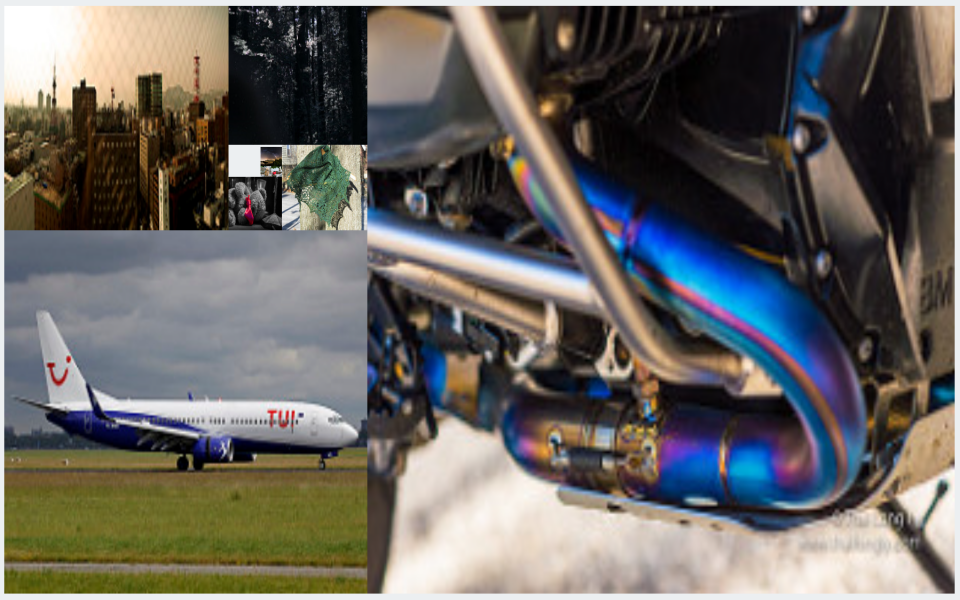
\includegraphics[width=\linewidth]{bluekittenflickr}
\caption[image spiral flickr]{image spiral flickr}
\label{fig:imgspiralflickr}
\end{figure}

For Getty the image search works slightly differently due to its \gls{api} restrictions. The query ``blue kitten'' gets turned into the word ``racy'' which then calls the \gls{api} to retrieve ten results (see below).

\begin{figure}[h!]
\centering
  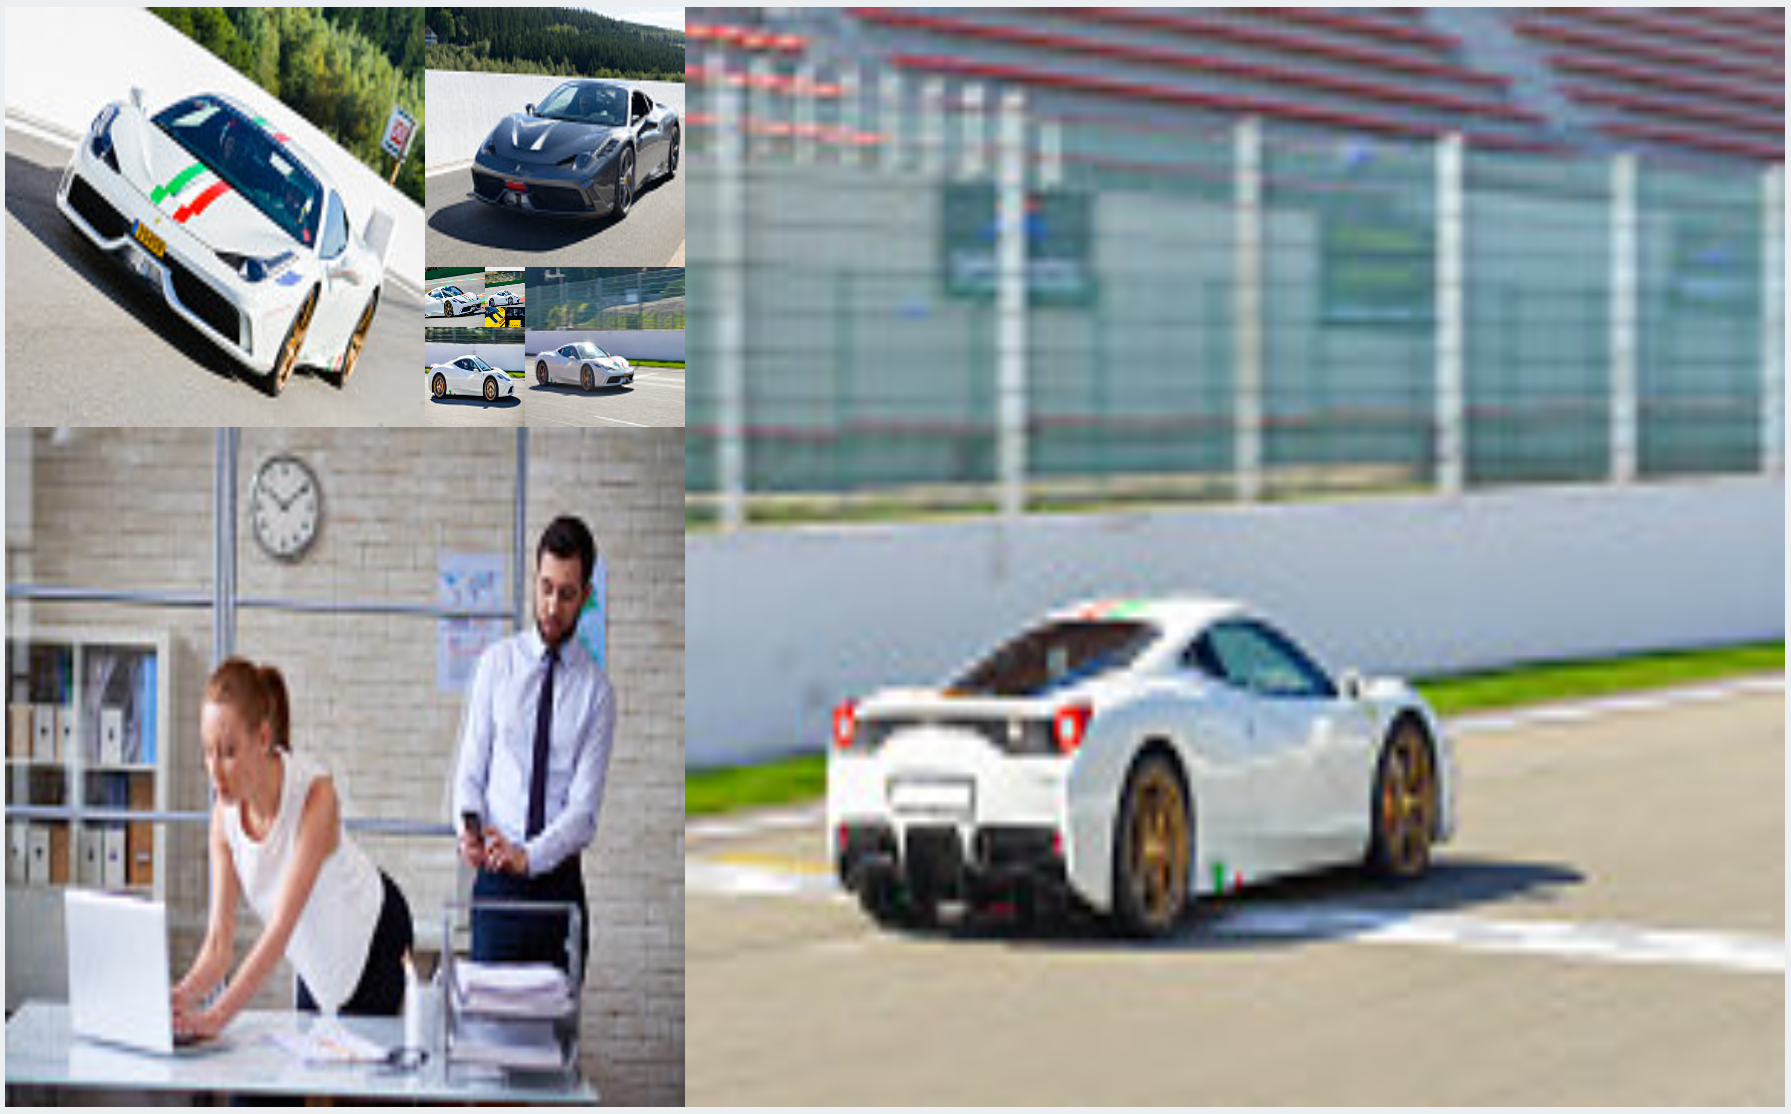
\includegraphics[width=\linewidth]{bluekittengetty}
\caption[image spiral getty]{image spiral getty}
\label{fig:imgspiralgetty}
\end{figure}

The difference is staggering.


\section{Design}

Content Perception\\
It is interesting to note how different the search results are perceived when presented in a different style (e.g. list rather than poem). This could be studied using focus groups using questionnaires and interviews or eye tracking tools to find out what users prefer or perceive as more creative for example.

\todo{poem vs list here}


\section{Meta}

\todo{add file for appendix with full git history}

On a different note, the project was completed over X years which includes an interruption and later on only a part time commitement.

I kept the project in a ``git repository''. Git is a version ontrol system that allows users to roll-back on changes and I further pushed my work to GitHub to make sure hardware failure or human error (i.e. lost or stolen property) would not affect my work. 

To understand git you need to know what commits are. They are the thing where I save my current state of the project and give it a description.

Below you can see a shortened version of the timeline of my commits between 20XX and the time of submission of this thesis. A full version can be found in appendix XYZ. You can see from this the time between programming work I did on \url{pata.physics.wtf} and its predecessors.


\todo{links to git and github}

\begin{verbatim}
  *   10f61f9  Sun 08 May 2016	 (HEAD -> api, origin/api) Merge remote-tracking branch 'refs/remotes/origin/master' into api
  |\  
  * | 71437f6  Tue 18 Aug 2015	 Flickr and Bing work, radio buttons work
  * | 6c552aa  Wed 12 Aug 2015	 Fixed image problem but not video.
  | | * 1cbb63d  Tue 11 Aug 2015	 (origin/thesis) Update textsurfer.py
  | |/  
  |/|   
  * | 0ebff0d  Tue 11 Aug 2015	 Analytics enabled again
  * | 703f977  Tue 11 Aug 2015	 Problems solved.
  * | 74a1fae  Tue 11 Aug 2015	 About to change l\_dict to dict of dict
  * | 0935b23  Mon 10 Aug 2015	 BUG FUCKER
  * | 4f7d91e  Mon 10 Aug 2015	 Turn debug off
  * | 58f0c2b  Mon 10 Aug 2015	 Button styling done
  * | 59add58  Mon 10 Aug 2015	 Email problem solved
  * |   f1b2d40  Sun 09 Aug 2015	 Merge branch 'Deploy' into thesis
  |\ \  
  | * | 435cb2d  Sun 09 Aug 2015	 Deployment works, added analytics
  | * | 8a63dc7  Sat 08 Aug 2015	 gunicorn runs locally fine.
  | * | 2861407  Sat 08 Aug 2015	 Revert 5f2c957..4026965
  | * | 4026965  Sat 08 Aug 2015	 Tests
  * | |   8f2eeab  Sat 08 Aug 2015	 Merge branch 'w3' into thesis
  |\ \ \  
  | |/ /  
  | * | 5f2c957  Sat 08 Aug 2015	 Stuff
  | * | 873153c  Fri 07 Aug 2015	 Tiny cleanup
  | * | 05d5760  Thu 06 Aug 2015	 Random Poems and Emailing works
  | * | 657126c  Wed 05 Aug 2015	 Random poems work - without links though
  | * | 3d31ea9  Wed 05 Aug 2015	 Randomise still only works once, count ok
  | * | 5f1d45b  Wed 05 Aug 2015	 Randomise poem works ONCE
  | * | c583341  Wed 05 Aug 2015	 Poem subtabs, email poems done
  | * | f1b3878  Wed 05 Aug 2015	 Hiding divs
  | * | a6939c4  Tue 04 Aug 2015	 huh?
  | * | e6b411d  Tue 04 Aug 2015	 Poem emails WORK Fuck YEAH!
  | * | 4b6b170  Tue 04 Aug 2015	 Test email
  | * | 24e356c  Tue 04 Aug 2015	 Better load icon
  | * | e6ae736  Tue 04 Aug 2015	 loading icon version 1
  | * | 51b43e2  Tue 04 Aug 2015	 Added 4th pictures
  | * | f2d8a83  Mon 03 Aug 2015	 Minor fixes
  * | |   1ddb03d  Mon 03 Aug 2015	 Merge branch 'w3' into thesis
  |\ \ \  
  | |/ /  
  | * | ca4eab3  Mon 03 Aug 2015	 Pretty good state.
  | * | 9370334  Mon 03 Aug 2015	 working on list display of images
  | * | e1f1ead  Mon 03 Aug 2015	 Stylesheets sorted and cleaned files
  * | |   9732d5b  Mon 03 Aug 2015	 Merge branch 'w3' into thesis
  |\ \ \  
  | |/ /  
\end{verbatim}

\spirals

I also kept the thesis under git version control. Since the thesis was written in \LaTeX you could almost say I `programmed' it. Below is an outline of the commit history for this thesis.

\begin{verbatim}
* 3f06260	 Edited readme again
* c721b33	 Edited readme
* ffbdb4b	 Edited readme
* 8870b3d	 Added gitignore file
* ba1a9c2	 Second commit
* 244c4b3	 First commit
\end{verbatim}







\section*{creative analysis}
\begin{draft}
  literary deconstruction and recombining to make new creative output? \\
  perception of results (poetry, source, algorithm) \\
  discuss applications from before (stimulates creative detour away from the obvious) \\

  How does this relate to Oulipo and Pataphysics? 

  Perhaps this is where I should talk a bit about the perception of results in their different output formats/styles. The poetry is automatically read with more gravity. Sorting by sources is a game of exploration or algorithms which becomes a game of finding the similarities within the result sets. They are different ways to view the same things and yet have a drastic influence of how the results are perceived. This also applies to the image and video search. Presenting results in spiral form is weird. Its hard to see where one image ends and another starts, they just kind of blur into each other. When listed as a list they immediately become more boring.

  talk abit about what the original plan was for some of the big changed elements in the website, e.g. the image search running 10 times on different keywords rather than running once with 10 results for the same keyword.
\end{draft}


DELETE EVERYTHING FROM BELOW HERE:


\begin{draft}
DELETE THIS

In this section we consider the possible uses and applications for the proposed creative search tool.

Our target audience is not quite as broad as that of a general search engine like Google. Instead, we aim to specifically cater for users who can appreciate creativity or users in need of creative inspiration. Users should generally be educated about the purpose of the search tool so that are not discouraged by what might appear to be nonsensical results. Users could include artists, writers or poets but equally anybody who is looking for out-of-the-box inspirations or simply a refreshingly different search engine to the standard.

The way we display and label results produced by the tool can influence how the user perceives them. The current prototype for example separates the results into its three components but we could have equally just mixed them all together. The less transparent the processes in the background (e.g.\ which algorithm was used, how does the result relate to the query precisely, etc.) are for the user, the more difficult it might be to appreciate the search.

There are many ways a pataphysical search tool could be used across disciplines.

In literature, for example, it could be used to write or generate poetry, either practically or as a simple aid for inspiration. We are not limited to poetry either; novels, librettos or plays could benefit from such pataphysicalised inspirations. One can imagine tools using this technology that let you explore books in a different ordering of sentences (a sort of pataphysical journey of paragraph hopping), tools that re-write poems or mix and match them together. Even our simple prototype shows potential in this area and could be even more powerful if we extended it to include more base texts, for example the whole set of books contained in Faustroll’s library ([20] and also [12]). A richer body of texts (by different authors) would produce a larger index which would possibly find many more matches through WordNet and end in a more varied list of results.

From a computer science perspective it could be used as one of the many algorithms used by traditional search engines for purposes like query feedback or expansion (e.g. “did you mean … “or “you might also be interested in … “). Depending on how creative we want the search engine to be, the higher we would rank the importance of this particular algorithm. One of the concepts related to the search tool, namely patadata, could have an impact on the development of the Semantic Web. Just as the Semantic Web is about organizing information semantically through objective metadata, patadata could be used to organize information pataphysically in a subjective way.

The prototype tool is already being used in the creation of an online opera, provisionally entitled from [place] to [place], created in collaboration with The Opera Group, an award-winning, nationally and internationally renowned opera company, specialising in commissioning and producing new operas. In particular, it is being used to create the libretto for one of the virtual islands whose navigation provides the central storyline for the opera. The opera will premiere in 2013, and will continue to develop thereafter, deploying new versions of the tool as they appear.
\end{draft}






\stopcontents[chapters]
